\documentclass[
10pt, % Main document font size
a4paper, % Paper type, use 'letterpaper' for US Letter paper
oneside, % One page layout (no page indentation)
%twoside, % Two page layout (page indentation for binding and different headers)
headinclude,footinclude, % Extra spacing for the header and footer
BCOR5mm, % Binding correction
]{scrartcl}

%%%%%%%%%%%%%%%%%%%%%%%%%%%%%%%%%%%%%%%%%
% Arsclassica Article
% Structure Specification File
%
% This file has been downloaded from:
% http://www.LaTeXTemplates.com
%
% Original author:
% Lorenzo Pantieri (http://www.lorenzopantieri.net) with extensive modifications by:
% Vel (vel@latextemplates.com)
%
% License:
% CC BY-NC-SA 3.0 (http://creativecommons.org/licenses/by-nc-sa/3.0/)
%
%%%%%%%%%%%%%%%%%%%%%%%%%%%%%%%%%%%%%%%%%

%----------------------------------------------------------------------------------------
%	REQUIRED PACKAGES
%----------------------------------------------------------------------------------------

\usepackage[
nochapters, % Turn off chapters since this is an article        
beramono, % Use the Bera Mono font for monospaced text (\texttt)
eulermath,% Use the Euler font for mathematics
pdfspacing, % Makes use of pdftex’ letter spacing capabilities via the microtype package
dottedtoc % Dotted lines leading to the page numbers in the table of contents
]{classicthesis} % The layout is based on the Classic Thesis style

\usepackage{arsclassica} % Modifies the Classic Thesis package

\usepackage[T1]{fontenc} % Use 8-bit encoding that has 256 glyphs

\usepackage[utf8]{inputenc} % Required for including letters with accents

\usepackage{graphicx} % Required for including images
\graphicspath{{Figures/}} % Set the default folder for images

\usepackage{enumitem} % Required for manipulating the whitespace between and within lists

\usepackage{lipsum} % Used for inserting dummy 'Lorem ipsum' text into the template

\usepackage{subfig} % Required for creating figures with multiple parts (subfigures)

\usepackage{amsmath,amssymb,amsthm} % For including math equations, theorems, symbols, etc

\usepackage{varioref} % More descriptive referencing

%----------------------------------------------------------------------------------------
%	THEOREM STYLES
%---------------------------------------------------------------------------------------

\theoremstyle{definition} % Define theorem styles here based on the definition style (used for definitions and examples)
\newtheorem{definition}{Definition}

\theoremstyle{plain} % Define theorem styles here based on the plain style (used for theorems, lemmas, propositions)
\newtheorem{theorem}{Theorem}

\theoremstyle{remark} % Define theorem styles here based on the remark style (used for remarks and notes)

%----------------------------------------------------------------------------------------
%	HYPERLINKS
%---------------------------------------------------------------------------------------

\hypersetup{
%draft, % Uncomment to remove all links (useful for printing in black and white)
colorlinks=true, breaklinks=true, bookmarks=true,bookmarksnumbered,
urlcolor=webbrown, linkcolor=RoyalBlue, citecolor=webgreen, % Link colors
pdftitle={}, % PDF title
pdfauthor={\textcopyright}, % PDF Author
pdfsubject={}, % PDF Subject
pdfkeywords={}, % PDF Keywords
pdfcreator={pdfLaTeX}, % PDF Creator
pdfproducer={LaTeX with hyperref and ClassicThesis} % PDF producer
}
\usepackage{cite}
\usepackage{adjustbox}
\usepackage{booktabs}
\hyphenation{Fortran hy-phen-ation} 
\captionsetup{font=footnotesize}
\usepackage{booktabs}
\usepackage{enumitem}
\usepackage{tabularx, makecell}%
\renewcommand\theadfont{\normalsize\bfseries}
        \usepackage{etoolbox} %
        \AtBeginEnvironment{tabularx}{\setlist[enumerate, 1]{wide, leftmargin=*, itemsep=0pt, before=\vspace{-\dimexpr\baselineskip +2 \partopsep}, after=\vspace{-\baselineskip}}}

%----------------------------------------------------------------------------------------
%	TITLE AND AUTHOR(S)
%----------------------------------------------------------------------------------------
\title{\normalfont\spacedallcaps{}} % The article title

%\author{\spacedlowsmallcaps{Fatemeh Hadi Nezhad\textsuperscript{1}}}

%\date{2019} % An optional date to appear under the author(s)

%----------------------------------------------------------------------------------------

\begin{document}

%----------------------------------------------------------------------------------------
%	HEADERS
%----------------------------------------------------------------------------------------

\renewcommand{\sectionmark}[1]{\markright{\spacedlowsmallcaps{#1}}} % The header for all pages 
\lehead{\mbox{\llap{\small\thepage\kern1em\color{halfgray} \vline}\color{halfgray}\hspace{0.5em}\rightmark\hfil}} % The header style

\pagestyle{scrheadings} % Enable the headers specified in this block

%----------------------------------------------------------------------------------------
%	TABLE OF CONTENTS & LISTS OF FIGURES AND TABLES
%----------------------------------------------------------------------------------------

%\maketitle % Print the title/author/date block

\setcounter{tocdepth}{3} % Set the depth of the table of contents to show sections and subsections only

\tableofcontents % Print the table of contents

%----------------------------------------------------------------------------------------
%	AUTHOR AFFILIATIONS
%----------------------------------------------------------------------------------------

%\let\thefootnote\relax\footnotetext{* \textit{Department of Quantitative System Biology, University of California, Merced, United States}}

%----------------------------------------------------------------------------------------

\newpage 

%----------------------------------------------------------------------------------------
%	Preparing Data
%----------------------------------------------------------------------------------------
\section{Introduction}
%------------------------------------------------
\section{Background}
% write this third 
% write a background for each aim
\subsection{TryTryp Genomes}	
\subsection{tRNA identity classifier}

%------------------------------------------------
\section{Specific Aims}
% write this first
\subsection{Developing a Eukaryotic tRNA identity classifier}
 
\begin{enumerate}[noitemsep] % [noitemsep] removes whitespace between the items for a compact look
\item Predict and annotate tRNA gene models from TriTryp genomes available on? TriTrypdb, a kinetoplastid genome database. 
\item Create a tRNA identity classifier based on Bayesian Networks that accepts phylogenetically structured data as input and outputs posterior probabilities of functional identities for query tRNA sequences.
\item Investigate anticodon shift/functional conversion events in tRNA genes of TryTrypDB, fly, yeast, worm, etc. 

\end{enumerate} 
\subsection{reconstructing ancestral rearrangements of tRNA gene clusters in eukaryotic genomes}
Develop algorithm(s) to reconstruct ancestral rearrangements of tRNA gene clusters in eukaryotic genomes, including functional conversions and genic sequence conversion events, and apply these to the above-named eukaryotic datasets to discover functionally converting genes in these datasets and predict boundaries of gene conversion events occurring in them. (I need to share with you the manuscript from Julie’s thesis on what we discovered in Drosophila, for you to fully see the significance of this proposed project). 
\subsection{Developing a machine learning framework to model the evolution of tRNA genes on an input phylogenetic tree}
Develop a machine learning framework to model the evolution of (either or both: {consensus structure, structure-function map}) tRNA genes on an input phylogenetic tree, and use this framework to improve alignment and gene-finding of evolutionarily diverse tRNA gene-sets.
%------------------------------------------------
\section{Approach}
\subsection{tRNA identity classifier}
% for each aim write an approach 

%------------------------------------------------
\section{Work to Date}
\subsection{Developing a Eukaryotic tRNA identity classifier}
 
\subsection{Predicting and annotating tRNA gene models}
From tritrypdb website, we downloaded the version 41 of 46 TryTryp genomes released on 2018-12-05.Genomes are compared based on number of sequence fragments relative to their length as shown in figure ~\vref{fig:gallery}. later, We annotated tRNA genes for the sequenced TryTryp genomes using two computational methods for tRNA prediction, tRNAscan-SE(ref) and Aragorn(ref). We integrated the result of both genefinders by keeping the union of tRNA gene predictions generated by tRNAscan-SE v2.0 using defult options (Lowe and Eddy 1997) and Aragorn v1.2.38 using options -i116 -t -br -seq -w -e -l -d (Laslett and Canback 2004). Genes with overlapped coordinate were considered as one gene. However, the identity and exact coordinate of both genefinders were saved seperately to be analysed later. Since these genefinders cannot predict initiators, we predicted the initiator tRNAs for the genes with anticodon 'CAT' from intersection of both tRNAscan (TSE) and Aragorn (ARA) Based on Conserved positions of initiators in Eukarya from the study by CHRISTIAN MARCK and HENRI GROSJEAN (ref?).

\begin{figure}[tb]
\centering 
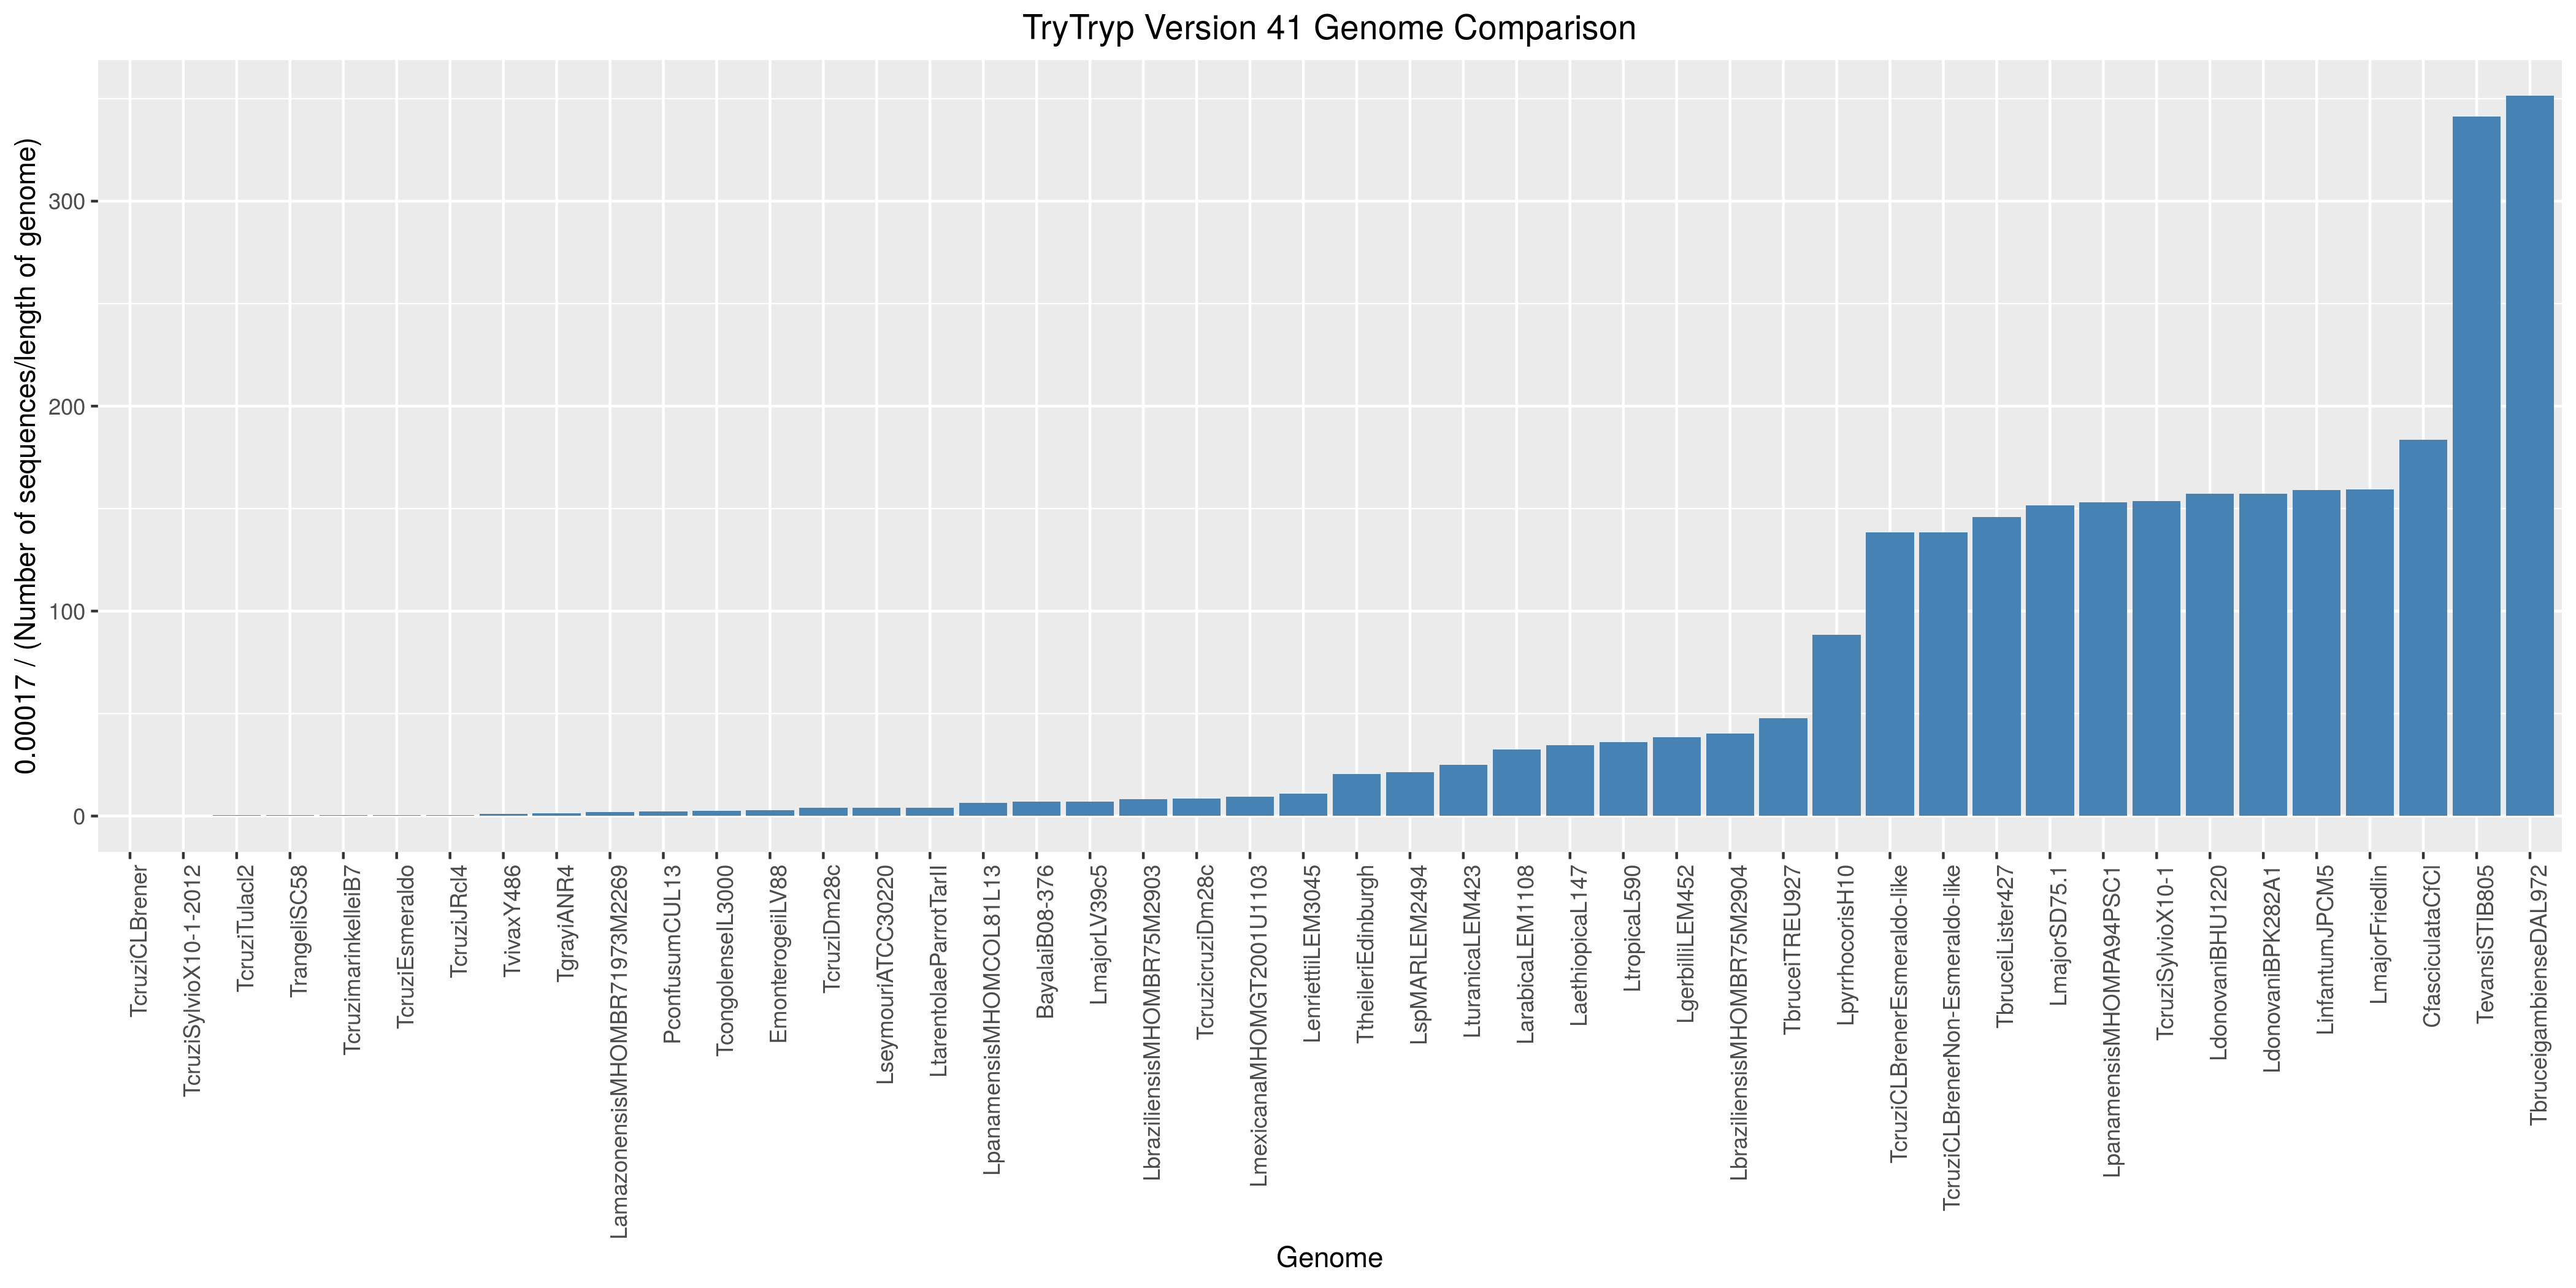
\includegraphics[width=0.8\columnwidth]{GenomeComparisonV41.png} 
\caption[Genome Comparison]{Comparing genomes based on formula ${(\frac{f(x)}{\max(f(x))})}^{-1}$. f(x) = Number of sequences in genome devided by the length of genome. The length of the bars shows how good the genomes are sequenced.} % The text in the square bracket is the caption for the list of figures while the text in the curly brackets is the figure caption
\label{fig:gallery} 
\end{figure}

\subsection{Summary of predicted TryTryp tRNA genes}
To investigate and compare tRNA genes predicted by two gene finders TSE and ARA, we made four sets of genes. Set one, TSE and ARA intersection, Set two, TSE and ARA union, Set three, genes found by ARA and Set four, genes found by TSE . For the intersection set, we dismissed genes which had different identity by ARA and TSE. for union set, for the porpuse of only making a summary of our genes, we picked TSE identity over ARA for overlapped genes. Table  ~\ref{table:2} shows a summary of these four sets. Further, to compare the coordinates of genes annotated by ARA and TSE we made a heatmap shown in figure ~\ref{fig:heatmap}. We see from this figure that the coordinates of same genes annotated by ARA and TSE do not always match. We then Analysed the reason for each set of displacement. Some of the main results of this analysis are:
1. Genes with same identity found by both genefindrs, usually have same reported structure, except for those with insertion or possible introns in their anticodon loop (ref). 2. ARA was seen to report up to 3 extra bases at the 3 prime end with many of them fallowing the pattern acc or ?cc, however, TSE reports only up to position 73. 4. few of the genes reported by Aragorn had Amino Acid arm one base longer than what TSE reports which caused a displacement at 5 prime end.
Further, to inspect whether our genefinders annotated tRNA genes of all 22 functional classes for each genome, we visualized the number of genes annotated for each genome in Figure ~\ref{fig:counts} and tRNA functional classes 	 by both TSE and ARA for each genome in Figure ~\ref{fig:types}.

\begin{table}[hbt]
\caption{summary of the predicted genes by TSE and ARA. We marked pseudo genes as \$, initiators as X, stop as \#, sup as "?", sec as Z and pyl as O}
\begin{adjustbox}{width=\columnwidth,center}
%\caption{Table of Grades}
%\centering
% make it as two table
\begin{tabular}{|l|lllllllllllllllllllllllllllllllllll|}
\hline
GeneSet & \# tRNA & \# nucleotides & N/T & gene length & \%G & \%C & \%T & \%A & \%intron & A & C & D & E & F & G & H & I & K & L & M & N & P & Q & R & S & T & V & W & Y & X & Z & \$ & ? & \# & O\\
TSE2 & 3631 & 270355 & 74.46 & 50-164 & 31.99 & 26.11 & 23.22 & 18.68 &  2.616 & 214 & 64 & 105 & 163 & 110 & 234 &  80 & 179 & 190 & 338 & 108 & 126 & 201 & 162 & 350 & 238 & 219 & 241 & 52 &  94 & 76 & 78 & 28 & 3 & 0 & 0\\
ARA & 4347 & 372539 & 85.70 & 70-215 & 32.64 & 26.92 & 22.87 & 17.57 & 14.677 & 257 & 86 & 124 & 193 & 125 & 339 & 129 & 213 & 194 & 393 & 101 & 153 & 228 & 175 & 420 & 362 & 248 & 282 & 60 &  90 & 76 & 82 &  0 & 0 & 2 & 4\\
UNION & 4381 & 377734 & 86.22 & 50-215 & 32.81 & 26.66 & 22.87 & 17.65 & 15.339 & 259 & 86 & 119 & 194 & 130 & 344 & 129 & 220 & 197 & 380 & 112 & 143 & 229 & 175 & 421 & 369 & 249 & 282 & 57 & 106 & 76 & 82 & 28 & 3 & 2 & 2\\
INTERSECTION & 3562 & 265160 & 74.44 & 68-89 & 32.01 & 26.13 & 23.22 & 18.64 &  2.330 & 212 & 64 & 105 & 162 & 105 & 229 &  80 & 172 & 187 & 338 &  97 & 125 & 200 & 162 & 349 & 230 & 218 & 241 & 52 &  78 & 76 & 78 &  6 & 0 & 0 & 0\\
\hline
\end{tabular}
\label{table:2}
\end{adjustbox}
\end{table}


\begin{figure}[tb]
\centering 
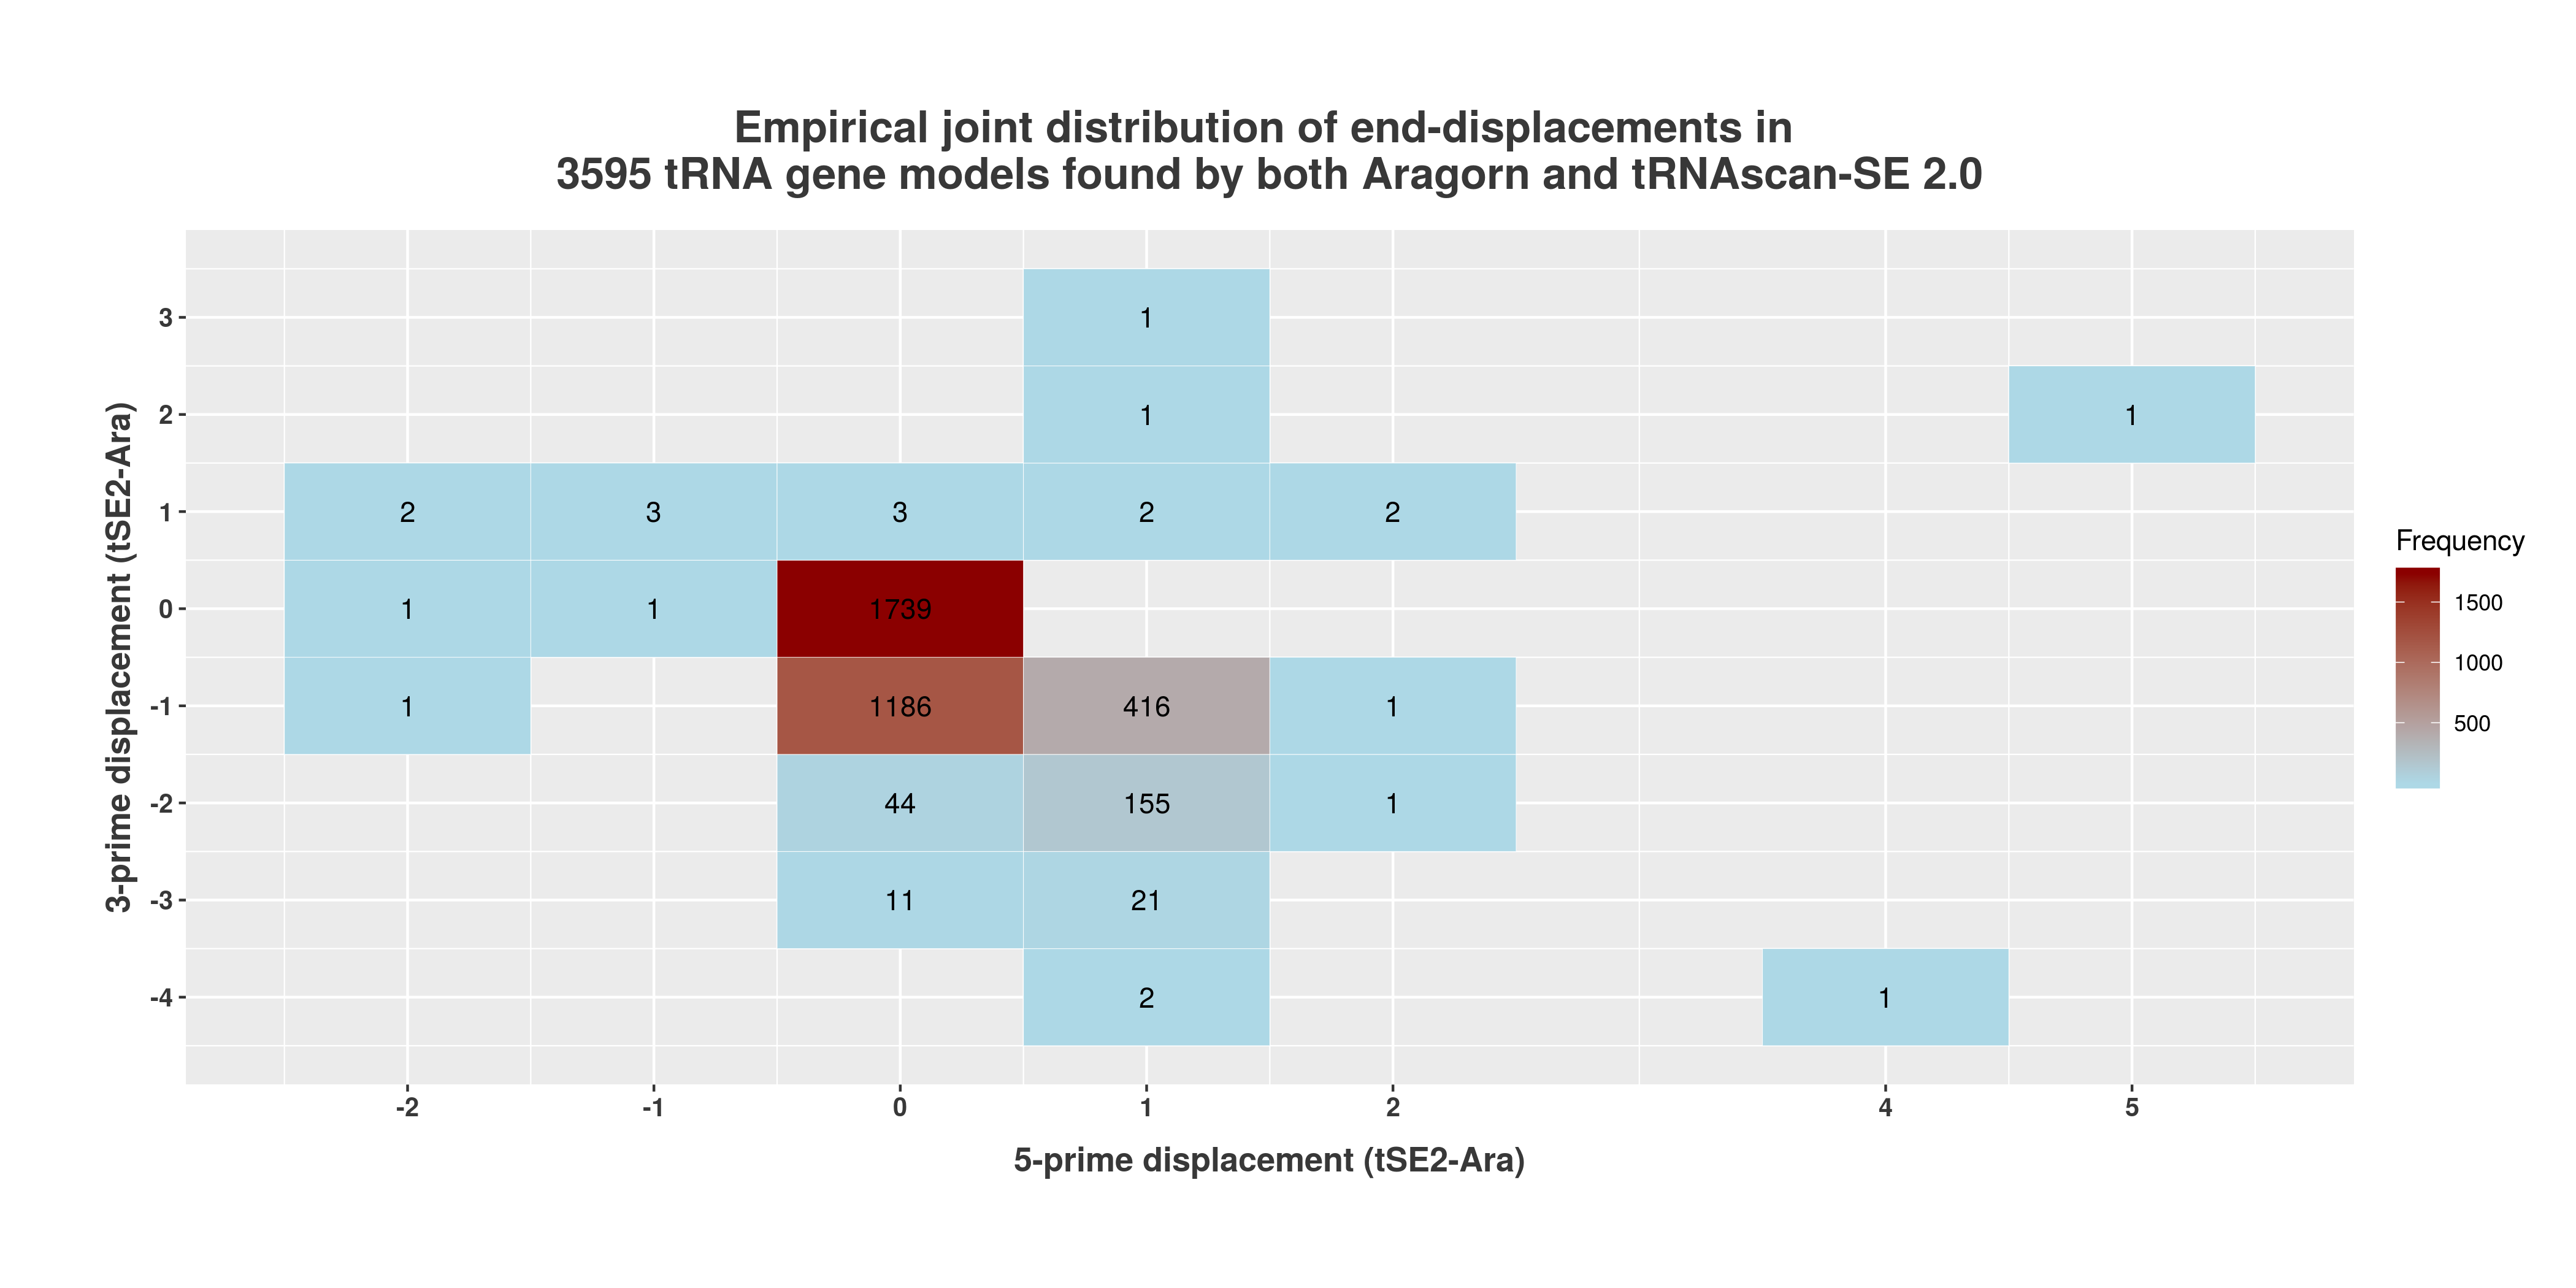
\includegraphics[width=0.8\columnwidth]{EndDisplacement.png} 
\caption[Genome Comparison]{Empirical joint distribution of end-displacements in ? tRNA gene models found by both Aragorn and tRNAscan-SE 2.0.} % The text in the square bracket is the caption for the list of figures while the text in the curly brackets is the figure caption
\label{fig:heatmap} 
\end{figure}
 
\begin{figure}[tb]
\centering 
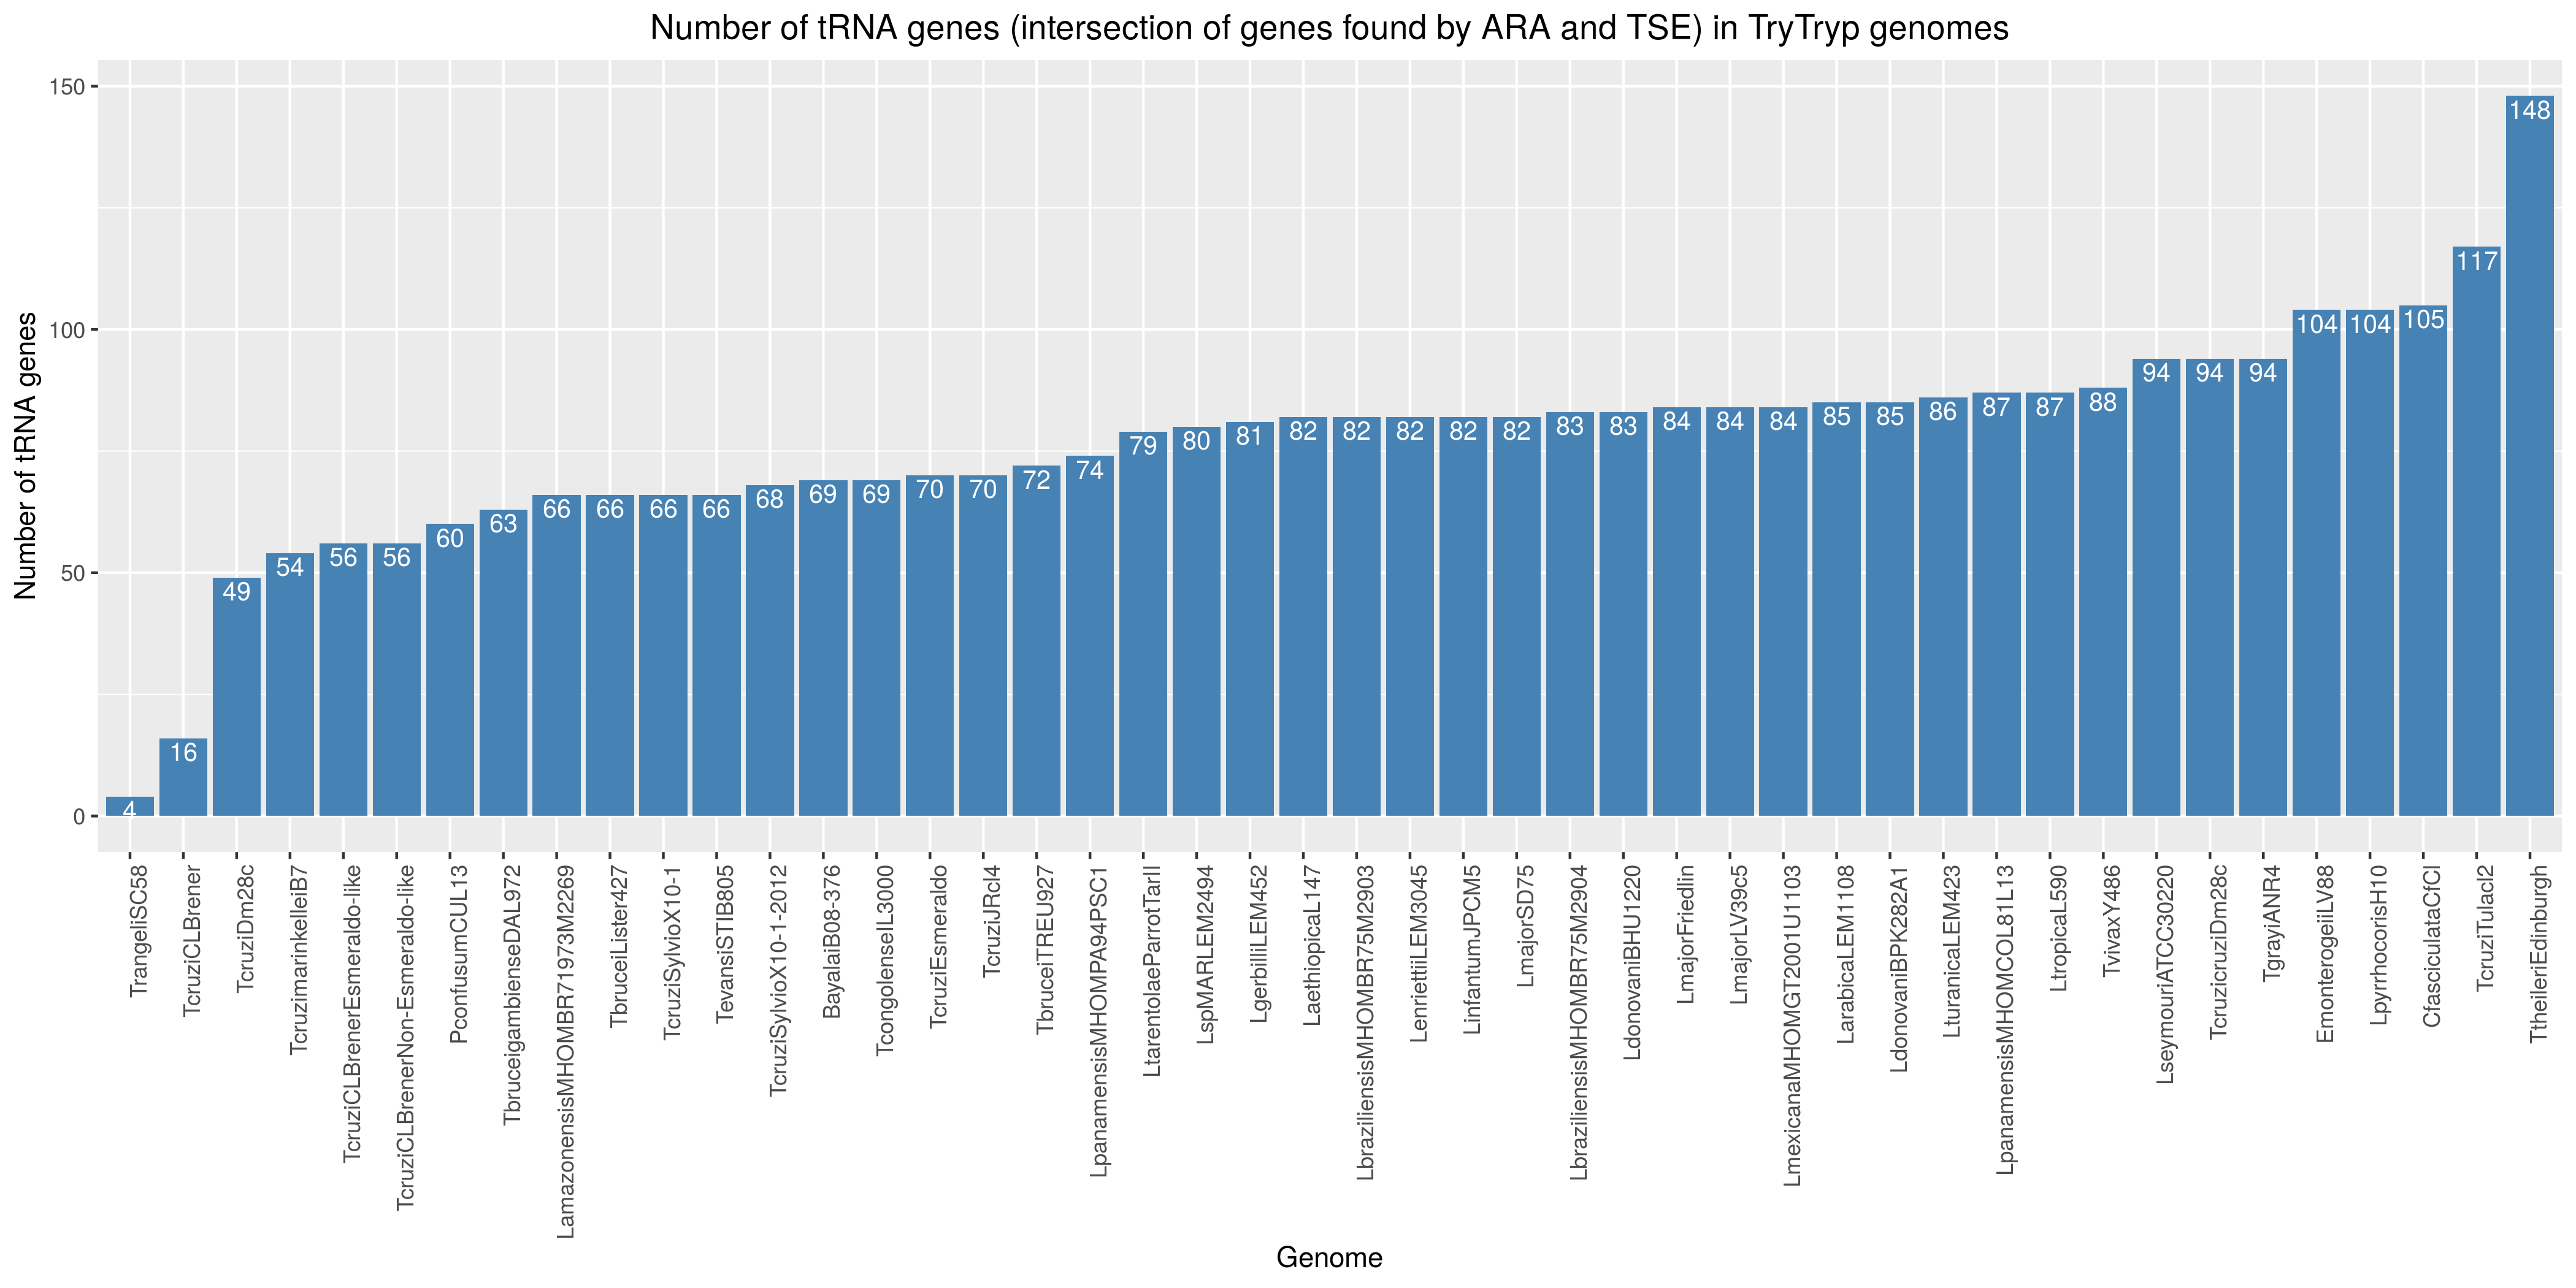
\includegraphics[width=0.8\columnwidth]{intersecttRNAcounts.png} 
\caption[Number of Genes annotated]{Number of genes annotated by both TSE and ARA for each TryTryp genome.} % The text in the square bracket is the caption for the list of figures while the text in the curly brackets is the figure caption
\label{fig:counts} 
\end{figure}

\begin{figure}[tb]
\centering 
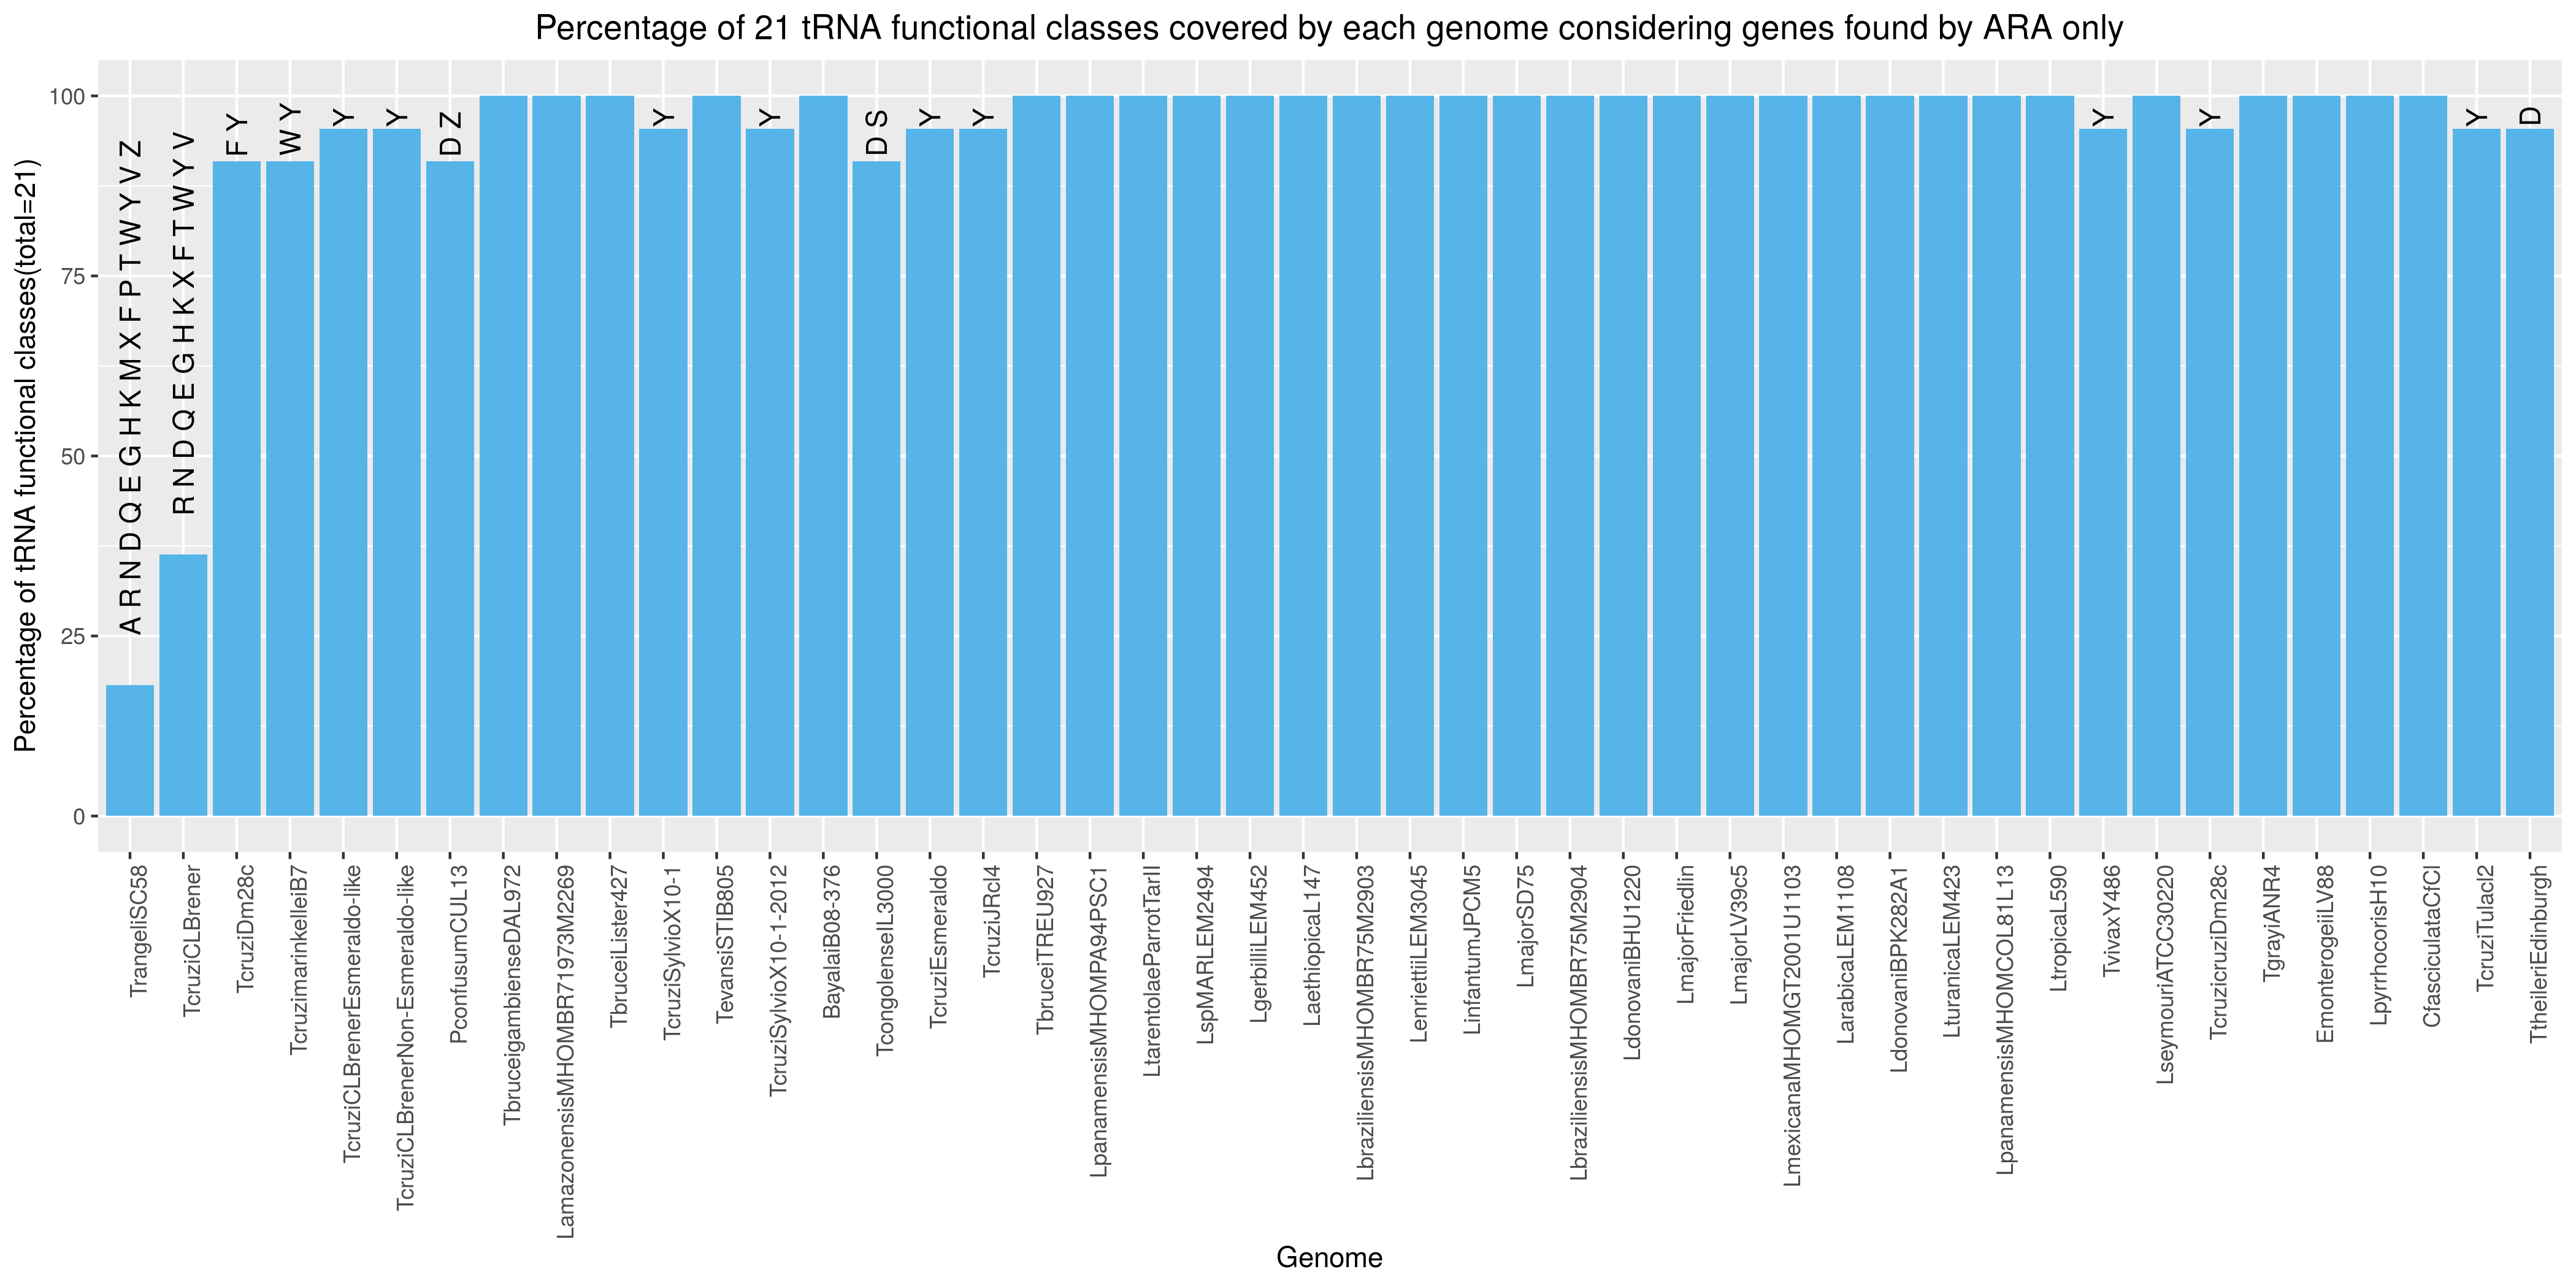
\includegraphics[width=0.8\columnwidth]{ara_funcPerc.png} 
\caption[Genome Comparison]{Percentage of 22 tRNA types annotated by both TSE and ARA for each TryTryp genomes. The label on top of each bar shows which tRNA classes are not annotated for the genome.} % The text in the square bracket is the caption for the list of figures while the text in the curly brackets is the figure caption
\label{fig:types} 
\end{figure}

\subsection{Creating an alignment pipline for TriTryp tRNA gene models}
to be able to compare tRNA gene sequences, we need to build a consensus tRNA gene model. To do so, I wrote a pipline which will accept our integrated gene file as input and returns a fasta file with genes aligned to together and a consensus structure which describes their folding pattern. The first step in this pipeline is to remove the varibale arms, introns and and other nucleotides in non-conserved positions using the secondary structures reported by our gene-finders. Second, we run covea v2.4.2 (Sean Eddy 1994) for the structural alignment of our genes based on the Eukaryotic model. Third, removing sites with more than 99\% gap, genes with more than 8 gaps in their aligned sequence, and genes with letter N in their sequence. at the end, we map the consensus structure to the standard numbering system (Sprinzl et al. 1991) (ref?).

\subsection{Creating an identity classifier for TriTryp tRNA gene models}
0.using the intersection set of our aligned gene files as training set
1.split the gene models based on their functional class, 
2.for each functional class, find the outlier using OD-seq and dismiss the outliers from training set
3.make profiles of each model class and score each sequence of our training set according to the log-odds of belonging to a specific functional class.
3.inspecting the distribution of our gene file. we would like to normalize the distribution of scores against each model to be able to use z-score of sequences scores against all profile models, and assign the best fit model it them.
4. after visualizing the distribution of score in the first round and inspecting the alignment of each model using an alignment viewer seaview(ref?), we saw that in each model tRNAs of specific genomes are better aligned to eachother than others. So, to investigate sub populations of our gene population in each model class... ? what ? 


\subsection{Finding potential Anti-codon shifts}
To find the potential anti-codon shifts, we calculated the z-score of the outliers from each model class against all the other models. for outlier with a relatively better z-score in another model class called ?, we compared the reported anti-codon for the genes to the possible anticodons of model ? to find the most possible shifts( shifts with the minimum numebr of substitution). later, we would like to verify these anti-codon shifts by using the synteny of gene clusters across closly related genomes (ref?).   

\subsection{identifying TriTryp-specific tRNA identity determinants in compare to Human tRNA genes}
We visualized differences in tRNA identity determinants between TryTryp and Human, and across TryTryp genomes, using four different Logos: 
\begin{enumerate}[noitemsep]

\item[1] Function Logos to estimate the potential identity determinants for each genome 
\item[2] Information Difference logos (ID logos), to show the evolutionary gain or loss of functional information between Human and TryTryp genomes 
\item[3] KullbackeLeibler divergence Difference logos (KLD logos) to show changes in the functional associations of features between Human and TryTryp genomes
\item[4] Using Three Logos mentioned above, we made bubble plots to show gains and shifts in functions of tRNAs in Trypanosomea contrasted against human tRNAs.

\end{enumerate}
Using phylogenetic trees of Trypanosoma from these works \cite{Souza:2018dg,Hughes:2003,Pothirat:2014,Kelly:2017}, we grouped TryTryp genomes as table \ref{table:4}. We excluded genome PconfusumCUL13 from the study, until we find a well sequenced version of this genome for which we can annotate all 22 functional classes of tRNAs. The Logo data for TryTryp genomes and Human can be found \href{https://github.com/fhadinezhadUC/Leishmania_2019/tree/master/Results/tsfmInput-output/output/Logos}{here}. you can find the bubble plots for each cluster \href{https://github.com/fhadinezhadUC/Leishmania_2019/tree/master/Results/tsfmInput-output/output/BubblePlots}{here}. we have 11 pages and each page has 21 models for all tRNA classes in a cluster. 
\begin{table}[hbt] 
\caption{Classification of TryTryp genomes. genomes not mentioned here are clustered as one genome.}
\begin{adjustbox}{width=\columnwidth,center}
\begin{tabular}{|c|c|c|c|c|c|c|c|}
        \toprule LenriettiComplex & AfricanTrypanosome & AmericanTrypanosome & Leishmania1 & Leishmania2 &LDonovaniComplex & LMexicanaComplex & Lvianna \\\midrule
        \parbox{.45\textwidth} {\begin{enumerate}
            \item LspMARLEM2494
            \item LenriettiiLEM3045
        \end{enumerate}} & \parbox{.45\textwidth}{\begin{enumerate}
            \item TbruceigambienseDAL972
            \item TbruceiLister427
            \item TbruceiTREU927
            \item TevansiSTIB805
            \item TcongolenseIL3000
            \item TvivaxY486
        \end{enumerate}} & \parbox{.45\textwidth}{\begin{enumerate}
            \item TgrayiANR4
            \item TrangeliSC58
            \item TcruziCLBrener
            \item TcruziCLBrenerEsmeraldo-like
            \item TcruziCLBrenerNon-Esmeraldo-like
            \item TcruzicruziDm28c
            \item TcruziDm28c
            \item TcruziEsmeraldo
            \item TcruziJRcl4
            \item TcruzimarinkelleiB7
            \item TcruziSylvioX10-1
            \item TcruziSylvioX10-1-2012
            \item TcruziTulacl2
            \item TtheileriEdinburgh
        \end{enumerate}} & \parbox{.45\textwidth}{\begin{enumerate}
            \item CfasciculataCfCl
            \item LseymouriATCC30220
            \item LpyrrhocorisH10
        \end{enumerate}}& \parbox{.45\textwidth}{\begin{enumerate}
            \item LmajorFriedlin
            \item LmajorLV39c5
            \item LmajorSD75
            \item LturanicaLEM423
            \item LarabicaLEM1108
            \item LtropicaL590
            \item LaethiopicaL147
            \item LgerbilliLEM452
        \end{enumerate}}& \parbox{.45\textwidth}{\begin{enumerate}
            \item LdonovaniBHU1220
            \item LdonovaniBPK282A1
            \item LinfantumJPCM5
        \end{enumerate}}& \parbox{.45\textwidth}{\begin{enumerate}
            \item Lamazonensis\\
                  MHOMBR71973M2269
            \item Lmexicana\\MHOMGT2001U1103
        \end{enumerate}}& \parbox{.45\textwidth}{\begin{enumerate}
            \item Lbraziliensis\\MHOMBR75M2904
            \item Lbraziliensis\\MHOMBR75M2903
            \item Lpanamensis\\MHOMPA94PSC1
            \item Lpanamensis\\MHOMCOL81L13
        \end{enumerate}}\\
        \bottomrule
\end{tabular}
\label{table:4}
\end{adjustbox}
\end{table}

Analysis of the output ... 
Do I need a picture of the logos here ? 

%------------------------------------------------
\section{Timeline and Milestones}
%------------------------------------------------
\section{Feasibility and Potential Pitfalls}
%------------------------------------------------
\section{Significance}

\subsection{tRNA identity classifier}
\subsection{Annotation of query tRNA genes}
Determining the identity of tRNA genes and creating a structure-function map of tRNA gene models is an open question which varies among diffrent species. Gene finders such tRNAscan-SE and Aragorn, will assign an identity to tRNA genes based on only anticodon sequence and they will not always agree on the location of anticodon sequence within anticodon loop, specitially when we have insertions or introns within the anticodon loop (reference the paper about the location of anticodon loop in eucaryiotic trna gene models). moreover, there is no complete set of identity determinants for trna genes of any species. Having a tRNA classifer which can find indetifies the identity determinant of a group of closely related species and assigns a functional class to them based on them will be robus to both anti-codon prediction error and sequence errors. TFAM (ref) one major tRNA classifier which classifies the function of tRNAs genes using sequence profile models, only provides bacterial tRNA identity models. It provides models for identifying only initiator in eukaryotic and archaeal. Also, tfam can only build models based on one cluster of tRNA models. Although, we may not always know the location of the genomes for which we want to classify tRNA genes in our phylogenetic tree. We would like to build a tRNA classifer which can take a phylogenetically structured data, build a consensus structure for each taxa, predicts the sonsensus structure for the ancestors and create taxa-specific models. Such classifer will help us to learn about the evolution of tRNAs. forexample, tRNAs of a genome may score better on the provides models for ancestor(inner nodes of tree) than it scores against the models made at the leave level of our tree. this can be hint of locating that genome in our phylogenetic tree.
such a classifer will help us to better annotate our predicted genes specially genes with unmatched identity between gene finders, genes found by only one of the genes, and genes marked as pseudo. A better annotation of our gene models will result in a better prediction of identity determinants, and better understand the changes of determinants across species. 

\subsection{Detecting possible anticodon shifts}
Anticodon is one of the major identity determinant in tRNAs. It is possible for a tRNA gene to switch to a different functional class after one or more mutations in its anticodon sequence and it has been shown to be possible in vitro as well (Schulman and Pelka 1989; Pallanck and Schulman 1991). mutations of bases in anticodon sequence resulting in change of tRNA’s amino acid charging is called alloaccepter shifts. relative number of anticodon shifts in a taxa can be the can suggest that tRNA gene redundancy is likely the driving factor (ref?)
also, by detecting the antocodon shifts, we can find sites with high covariation with anticodon shifts as potential determinants of tRNAs.\\ 
Previous works on anticodon shifts in eukaryotic tRNA genes (ref) has been done using a synteny-conservation-based method which looks for different anticodons within ortholog tRNAs as potential anticodon shifts. although this method is .... Mappings of flanking regions for each tRNA agains all other flanking regions and and ortholog set compilation may not be computationally efficient. By building a tRNA classifer we can score all the query tRNAs against all the models with time complexity of length of query. further, tRNA gene models with mismatch identity assigned by the classifier and the identity assigned by genefinders based on anti-codon, can be used as the potential anticodon shifts. these quences can be further be used in flank-mapping method for the perpuse of verification. 


\subsection{Detecting differences of indentity determinants between Trypanosoma and Human tRNA genes}

   4. the result of gene annotation can be used in detection of differenced in identity determinants of Human and Trypanosoma parasite. 

what is the gap for each of the mentioned points above?

papers related and the gaps: 
tfam: for procariouts. why can't we use it for eukariots. 


% write the significance of each aim
%----------------------------------------------------------------------------------------
%	BIBLIOGRAPHYyour own dat
%----------------------------------------------------------------------------------------
\newpage
\renewcommand{\refname}{\spacedlowsmallcaps{References}} % For modifying the bibliography heading

\bibliographystyle{unsrt}

\bibliography{sample.bib} % The file containing the bibliography

%----------------------------------------------------------------------------------------

\end{document}